% =====================================================================
%  Shared figure floats — 共享图件
%  供 main.tex / main_oup.tex / preprint.tex 共同 \input。
%  图注自洽；图内元素英文标注；改动图注只需改这一处，不会在三版之间漂移。
%  Shared figure float definitions for all three builds. Edit a caption here
%  once and every build picks it up; no per-build drift.
% =====================================================================

\begin{figure*}[t]
\centering
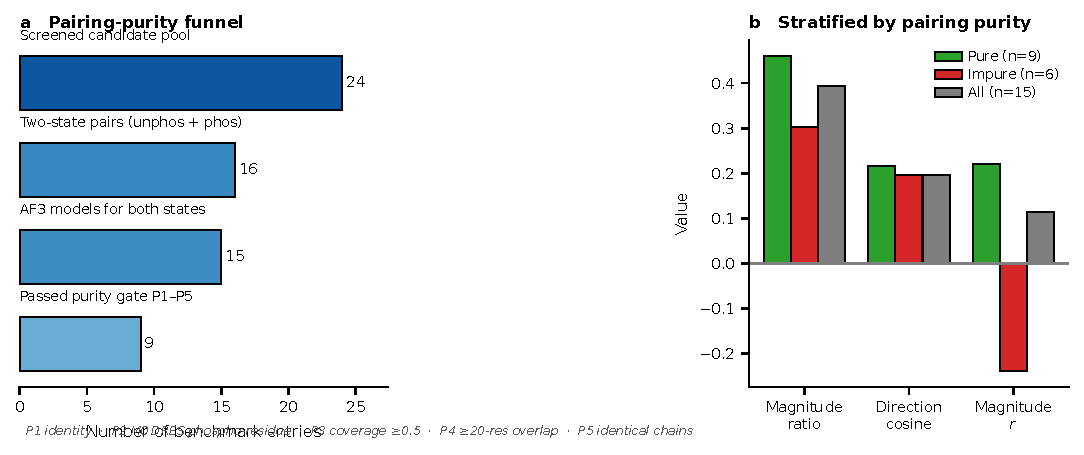
\includegraphics[width=\textwidth]{Fig1_purity_funnel.pdf}
\caption{\textbf{Pairing purity shapes the benchmark and the conclusion.}
(a) Funnel from the screened candidate pool through the two-state and
AF3-availability filters to the pairs passing the P1--P5 purity gate.
(b) The same frozen per-protein results stratified by pairing purity,
showing the median amplitude ratio, median direction cosine and magnitude
correlation for pure ($n=9$), impure ($n=6$) and all ($n=15$) pairs.
Purity here means chain-composition matching (P5), not ligand matching: the
nine pure pairs are not identical apart from the phosphate, and two of them
carry engineered substitutions (AURKA T287D, one residue from the site;
PAK1 K299R, present in both states); a further pair outside the pure
stratum (IKBKB) uses an S177E/S181E phosphomimetic non-phospho reference.
See Sec.~\ref{sec:purity} and the confound audit shipped with the data.}
\label{fig:funnel}
\end{figure*}

\begin{figure*}[t]
\centering
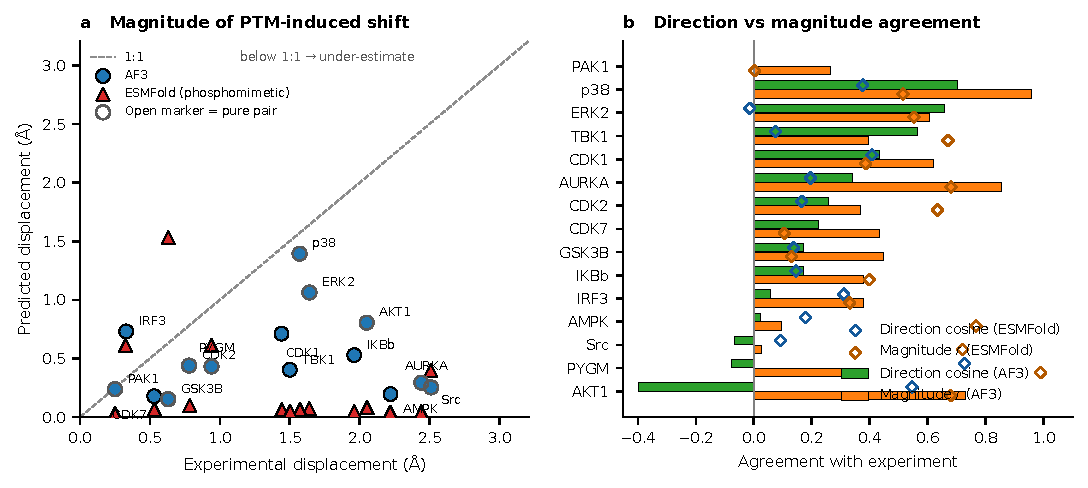
\includegraphics[width=\textwidth]{Fig2_af3_vs_pdb.pdf}
\caption{\textbf{Predicted versus experimental phosphorylation-induced
displacement.} (a) Per-protein mean experimental displacement against the
predicted displacement for AF3 (circles) and ESMFold with a phosphomimetic
phospho state (triangles); the dashed line is $1{:}1$. Open markers denote
purely paired structures. (b) Per-protein direction cosine and magnitude
correlation for AF3 (bars) and ESMFold (diamonds). Neither predictor's
displacement tracks the experimental one.}
\label{fig:fig2}
\end{figure*}

\begin{figure*}[t]
\centering
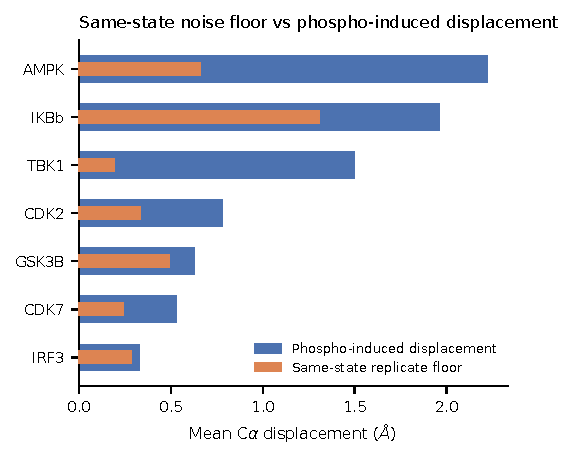
\includegraphics[width=\textwidth]{FigS1_noise_floor.pdf}
\caption{\textbf{Same-state noise floor.} Experimental same-state
dispersion (crystallographically independent copies) and predictor
same-state dispersion (across AF3 models) compared with the
phosphorylation-induced experimental displacement.}
\label{fig:noise}
\end{figure*}

\begin{figure*}[t]
\centering
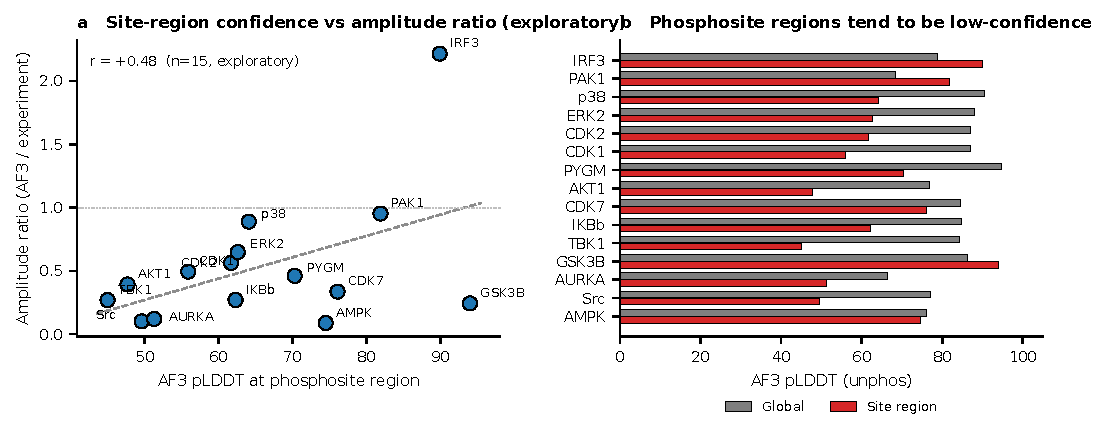
\includegraphics[width=\textwidth]{Fig4_plddt_vs_amplitude.pdf}
\caption{\textbf{Site pLDDT and agreement.} (a) Site-region pLDDT against
amplitude ratio for the 15 pairs (labelled), with a least-squares fit; the
apparent association is carried by IRF3 and collapses when it is removed
(Sec.~\ref{sec:res-confidence}). (b) Site-region versus global pLDDT,
showing that phosphosite regions tend to be lower-confidence than the rest
of the chain.}
\label{fig:plddt}
\end{figure*}

\begin{figure*}[t]
\centering
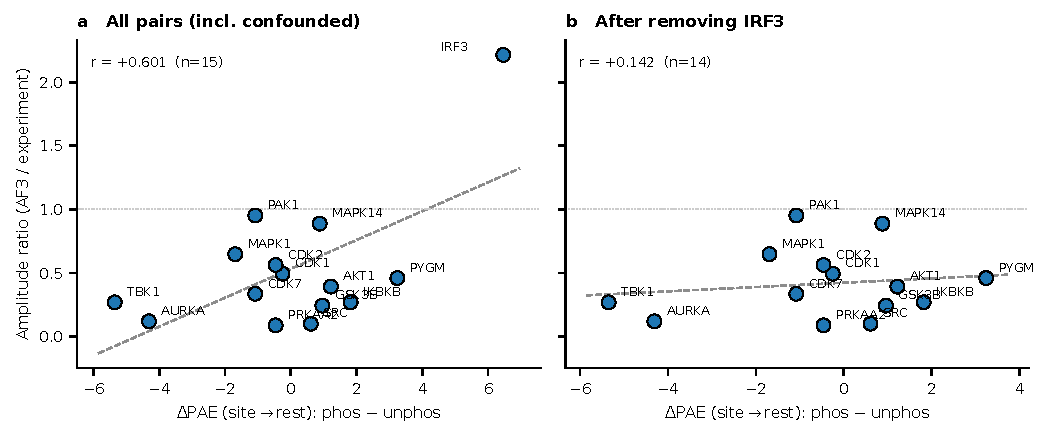
\includegraphics[width=\textwidth]{Fig5_pae_leverage.pdf}
\caption{\textbf{$\Delta$PAE association is a single-point effect.}
$\Delta$PAE (site$\rightarrow$rest) against amplitude ratio, all pairs
(left) and after removing IRF3 (right).}
\label{fig:pae}
\end{figure*}

\begin{figure*}[t]
\centering
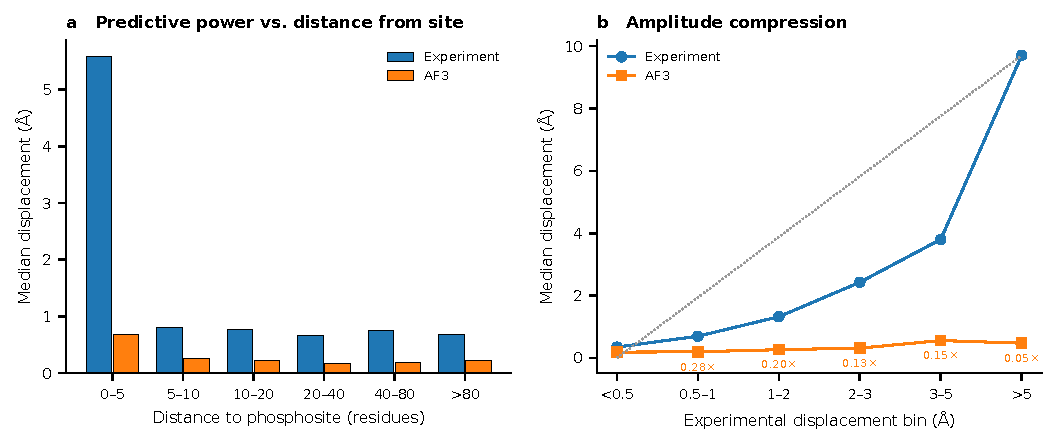
\includegraphics[width=\textwidth]{Fig3_residue_spectrum.pdf}
\caption{\textbf{Residue-level response saturates.} Median
predicted/experimental displacement ratio as a function of experimental
displacement magnitude, over all 5{,}148 common residues across the 15
cohort proteins; the decline is monotone across the six bins. The analysis
uses the first AF3 model of each state (model 0), not a multi-model average.
A distance decomposition of the same residues shows no trend
(Sec.~\ref{sec:res-explore}).}
\label{fig:spectrum}
\end{figure*}
